After a taxi driver activates the taxi service, he can receive a notification request for a taxi ride. He can accept or refuse the request. If the request is accepted, he has to go to the origin location indicated in the notification.


\subparagraph{Functional requirements}
\noindent
    \begin{itemize}
        \item After the taxi driver receives a notification, if the system does not receive an answer within 1 minute, the notification is passed to the following driver in the taxi queue.
        \item If there are no available taxi drivers in a city zone, the system looks for an available taxi for a maximum of 10 times. 
        \item If the system can not find an available taxi, it sends a notification of failure to the user.
        \item When the taxi reaches the origin zone, the system asks him to confirm the begin of the ride.
        \item When the taxi reaches the destination zone, the system asks him to confirm the end of the ride.
        \item After the taxi driver confirms the begin of a ride, the system sets his status to 'busy'.
        \item After the taxi driver confirms the end of a ride, the system sets his status to 'available'.
        \item When a ride is completed, the system stores the data of the ride into the DB.
    \end{itemize}
    
\begin{figure}[H]
    \centering
    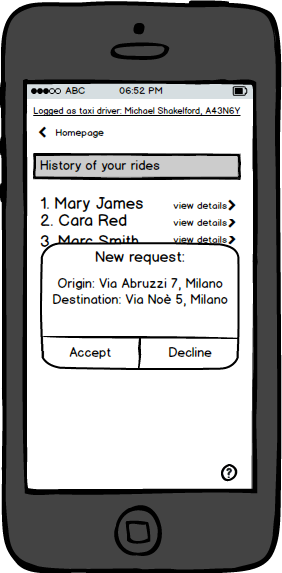
\includegraphics[width=5cm]{./Mockups/RequestHandling.png}
    \caption{Notification request incoming}
\end{figure}
